\documentclass[a4paper, titlepage]{article}

\usepackage[utf8]{inputenc}
\usepackage[T1]{fontenc}
\usepackage[ngerman]{babel}
\usepackage{graphicx}
\usepackage{hyperref}
\hypersetup{
    colorlinks=true,
    linkcolor=black,
    filecolor=magenta,      
    urlcolor=cyan,
}

\title{React Replacinator}
\author{Damien Flury, Aaron Stampa}
\date{24. Juni 2020}

\begin{document}
  \maketitle
  \abstract{Dies ist ein React Projekt, welches im
  Rahmen des ÜK-Moduls \glqq{}Webtechnologien clientseitig anwenden\grqq{}
  entstanden ist.}
  \tableofcontents
  \newpage
  \section{Einleitung}
  sdfokjsdfjks
  \section{Versionsverwaltung}
  Zur Versionsverwaltung haben wir Github verwendet.
  Darin haben wir mit GitHub Projects gearbeitet,
  um unsere Tasks übersichtlich verwalten zu
  können. Das Repository ist unter 
  \href{https://github.com/DamienFlury/react-replacinator}{React Replacinator}
  verfügbar. In Abbildung \ref{git:commit-history} finden Sie einen Screenshot
  der Commit History.

  \begin{figure}
    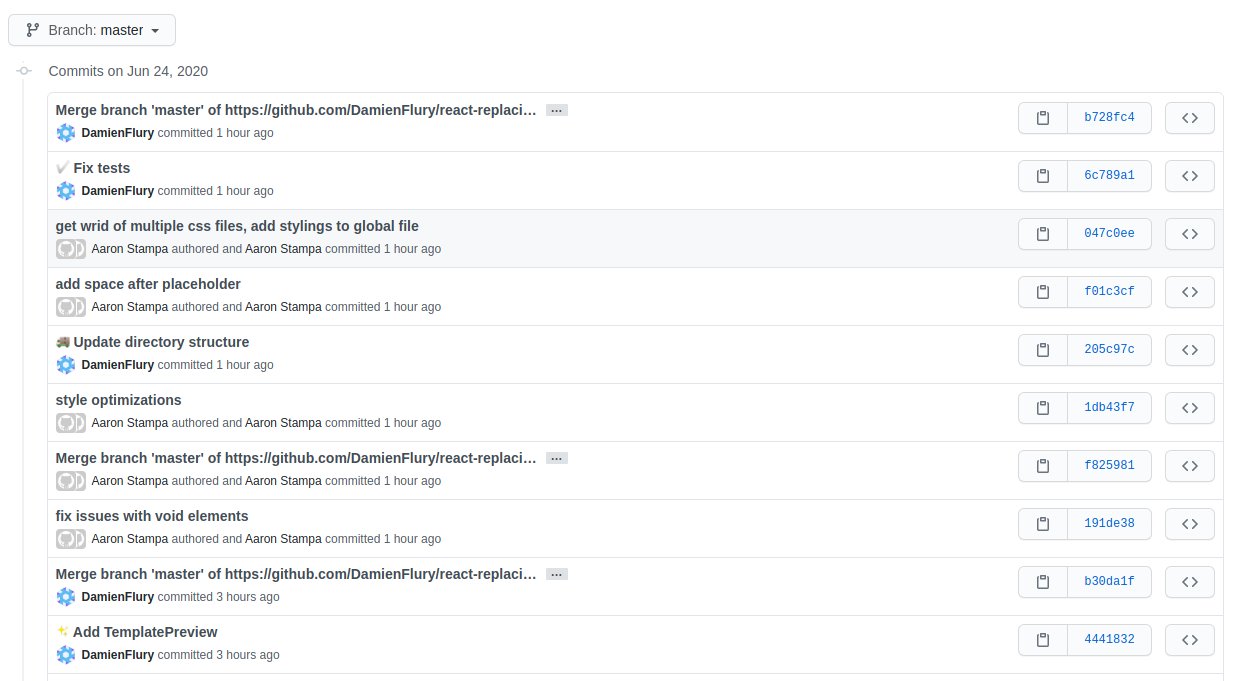
\includegraphics[width=\textwidth]{images/commit-history.png}
    \caption{Commit History}
    \label{git:commit-history}
  \end{figure}
  \section{Idee}
  Die Idee für unser Projekt kam von unserem ÜK-Leiter, der uns mitteilte, 
  lange nach einem Komponenten dieser Art gesucht und noch nichts passendes 
  dazugefunden hat. 
  Es handelt sich hierbei um eine wiederverwendbare Komponente, mit der man 
  Emailvorlagen erstellen kann. Es soll möglich sein, vorgegebene Platzhalter 
  via WYSIWYG in einen Emailtext mit einfachen Klicks einzubinden. 
  Ausserdem soll es eine Preview des fertigen Mails geben.
  \subsection{Komponenten Diagramm}
\end{document}